\subsection{Creating a Session}
The structure of the Sessions component is similar to the Questions component. There is a list of sessions that is kept up to date when a session is added, edited or deleted. A session contains a list of questions that are stored in a separate database table linking the Question and Session tables. This ensures the possibility of adding a question to multiple sessions, and that an answer does not affect the statistic of another session.

\begin{figure}[H]
	\centering
	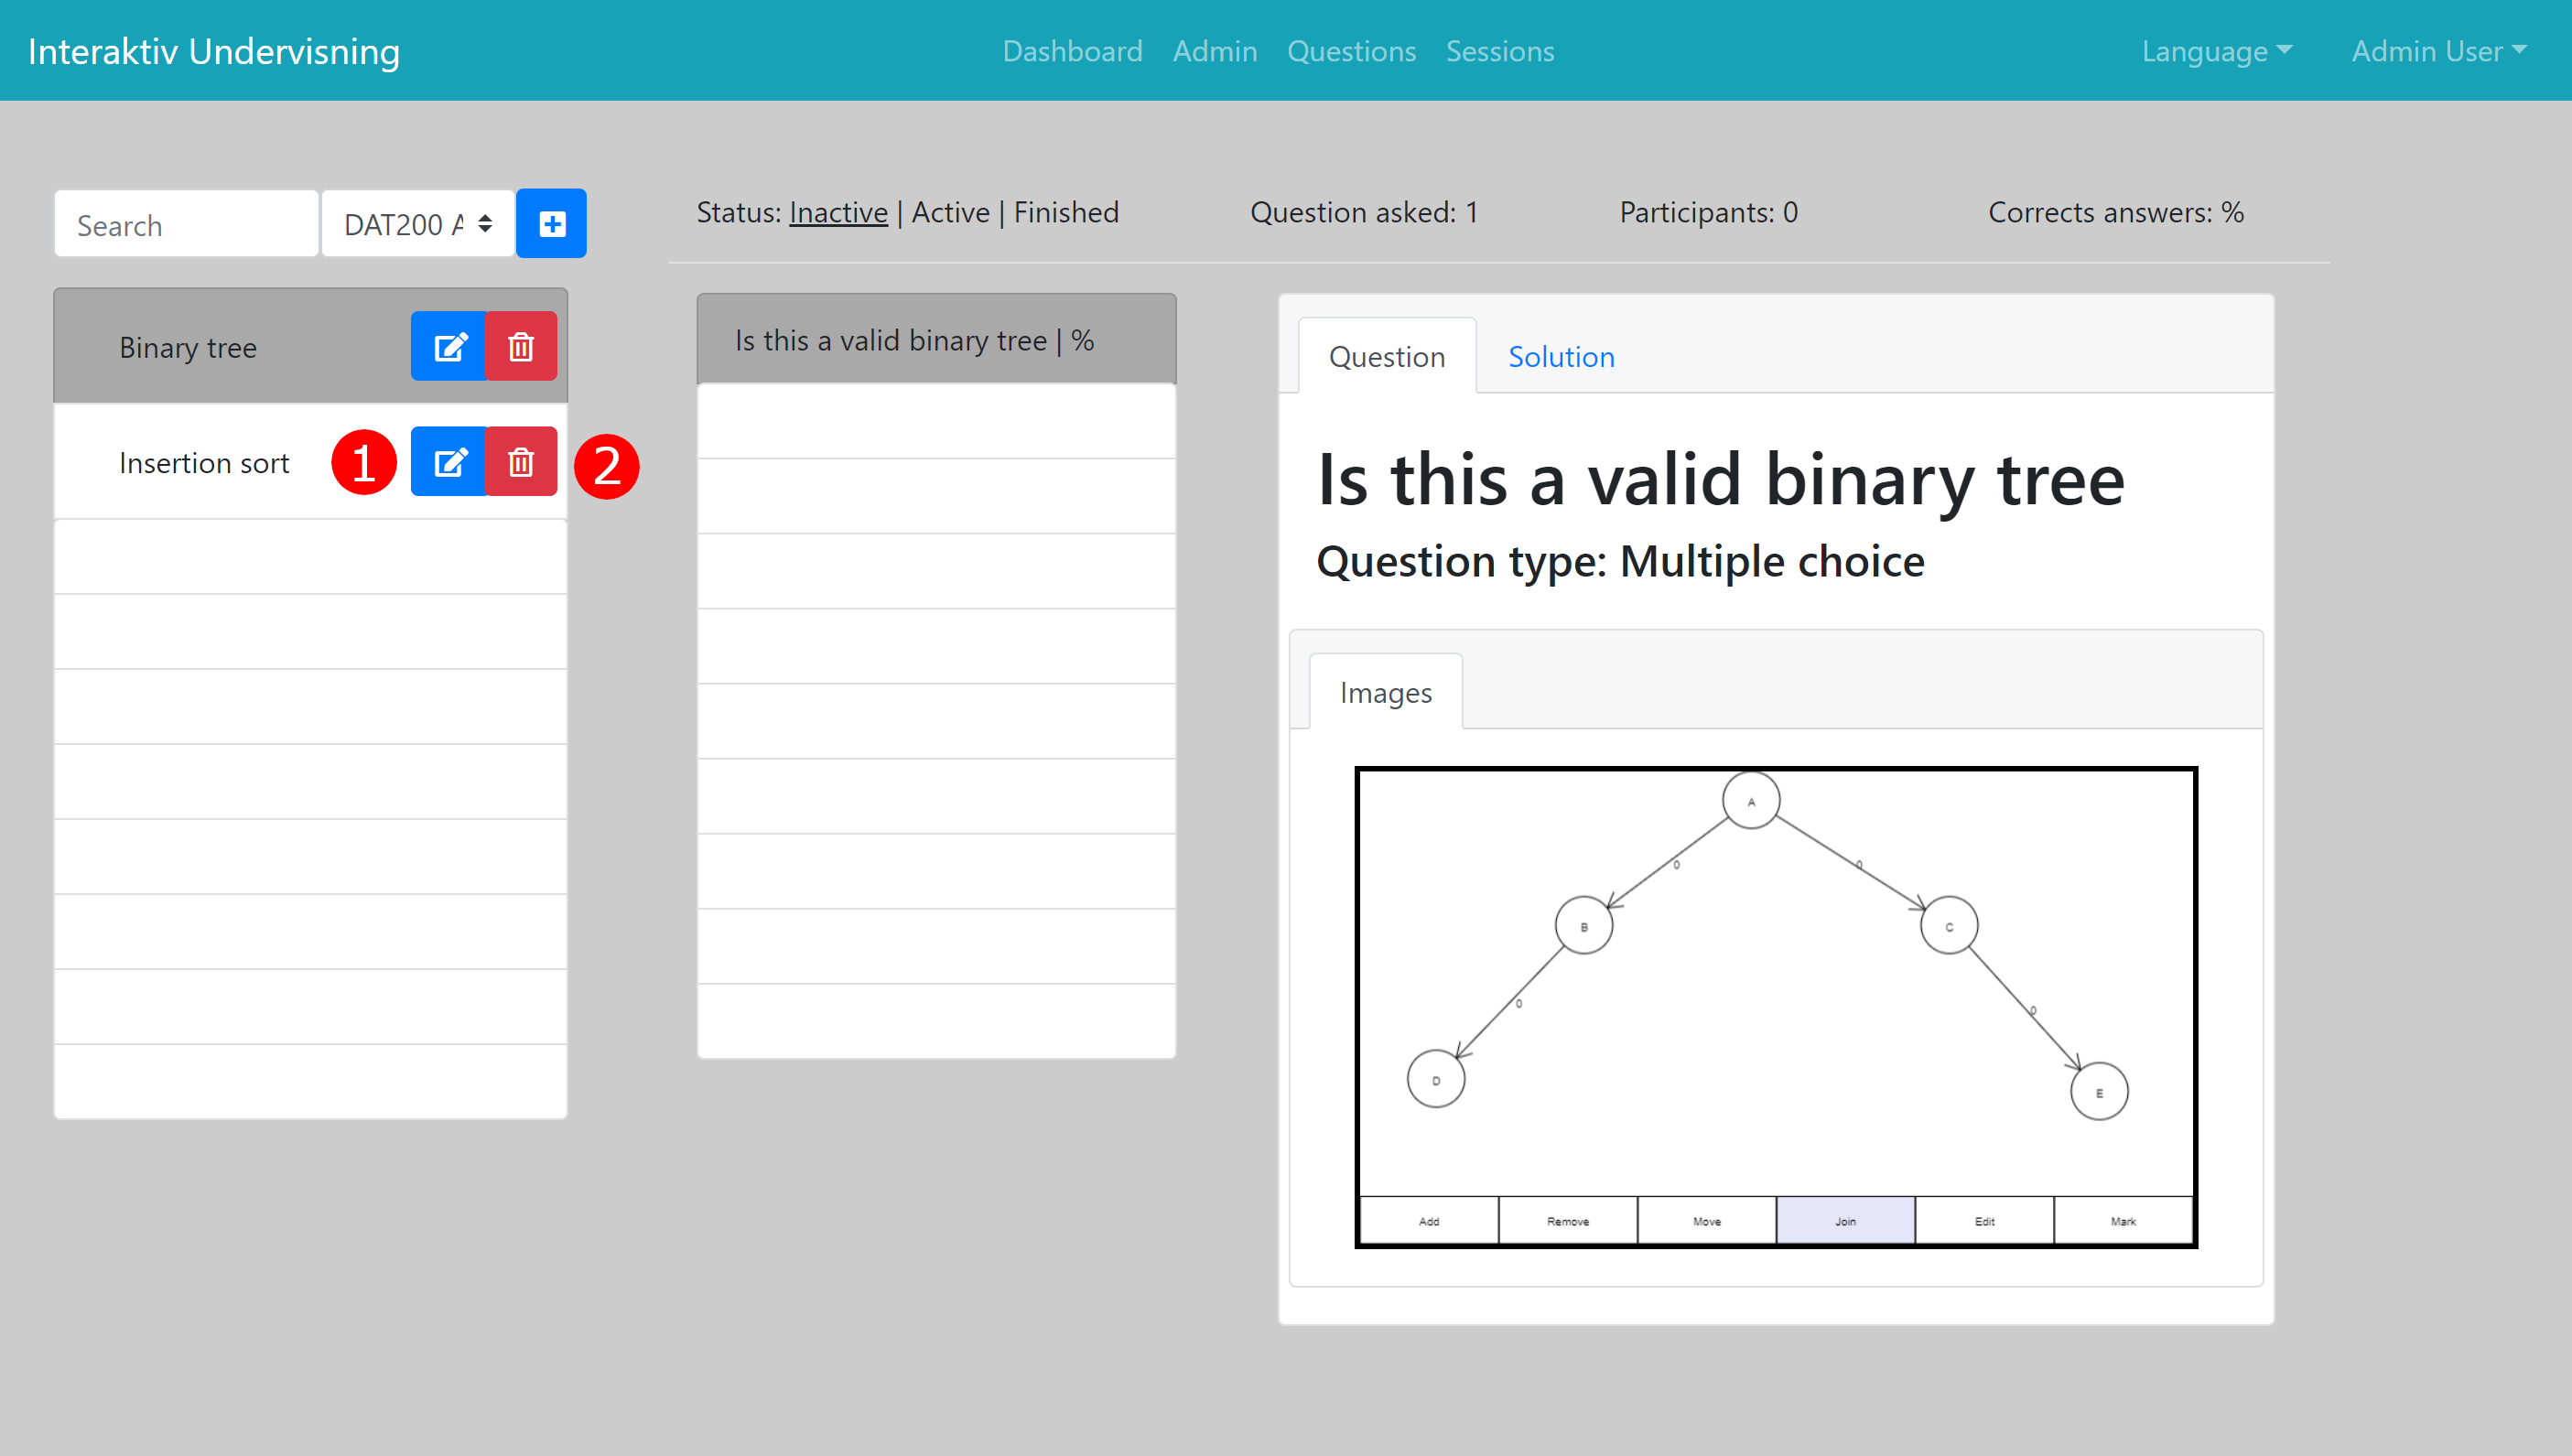
\includegraphics[width=0.80\linewidth]{/userManual/admin/sessionsWithSessions}
	\label{fig:sessionPage}
	\caption{This figure displays the Session component.}
\end{figure}